% !TeX spellcheck = en_US
\documentclass[12pt, a4paper]{book}
\usepackage[utf8]{inputenc}
\usepackage[english,vietnamese]{babel}

\setlength{\parskip}{0.5\baselineskip}%
\setlength{\parindent}{0pt}%
% Set the title of the current document to be produced.
\newcommand{\doctitle}{{{\Huge \textbf{Data Mesh Architecture}}}}
% Command for the due date of the homework.
%\newcommand{\duedate}{\color{rltred}{\faCalendarCheckO { }Due date: May 1st, before midnight \faCalendarCheckO	}}

%------------------------------------------------------------
% Import commands for both teacher and course information.  | 
% NOTE: Change your teacher and course info in these files. |
%------>------>------>------>------>------>------>------>-->|
%-------------------------------------------------
% Teacher-specific commands                      |
%---------------                                 |
%-> Instructions: change your teacher info here. |
%------->------>------>------>------>------>---->|
%
\newcommand{\instructor}{Thanh C. Nguyen}
\newcommand{\office}{Office number}
\newcommand{\hours}{By appointment}
\newcommand{\phone}{0}
\newcommand{\college}{\textbf{Viettel Group - Viettel Digital Talent Program}}
\newcommand{\email}{thanhnc221@viettel.com.vn}
\newcommand{\faculty}{Viettel Group}
\newcommand{\department}{Information Technology Division}
                              %|
%-------------------------------------------------
% Course-specific commands                       |
%---------------                                 |
%-> Instructions: change your course info here.  |
%------->------>------>------>------>------>---->|
%
\newcommand{\semester}{2022.2}
\newcommand{\csection}{00001 \& 00002}
\newcommand{\ponderation}{2-4-3 (Theory-Lab-Homework)}
\newcommand{\coursetitle}{Data Mesh Architecture}
\newcommand{\coursenumber}{\textbf{VDT2023-SDE}}
\newcommand{\prerequisite}{All porgram courses semesters 1-4}
                               %|   
%
%------------------------------------------------------------
%-- Import packages and custom command definitons.          |
%------>------>------>------>------>------>------>------>-->|
%----------------------------------------------------
% The following is a list of LaTeX packages imports |
%------->------>------>------>------>------>---->---|
%

% The margins at the bottom of the page has been reduced.
% this allows for a slim footer.
\usepackage[left=2cm,right=2cm,top=2cm,bottom=2cm]{geometry}
% Original size:
%\usepackage[inner=1.5cm,outer=1.5cm,top=1.5cm,bottom=.5cm,margin=1in]{geometry}
\usepackage[
    colorlinks,
    %pagebackref,
    pdfusetitle,
    urlcolor=blue,
    citecolor=blue,
    linkcolor=blue,    
    plainpages=false]
{hyperref}            
% ftp://ftp.dante.de/tex-archive/fonts/bbding/bbding.pdf
%https://ctan.math.illinois.edu/fonts/bbding/bbding.pdf
\usepackage{fancyhdr, lastpage, bbding, pmboxdraw}
\usepackage{fancyvrb}
\usepackage{bigints}
\PassOptionsToPackage{usenames,dvipsnames}{xcolor}
\usepackage{graphicx,wrapfig,lipsum}
\usepackage{acronym}
\usepackage{amsthm}
\usepackage{amssymb}
\usepackage{amsmath}
\usepackage{caption}
\usepackage{xcolor}
\usepackage{bigints}
\usepackage{enumitem}
\usepackage{tabularx}
\usepackage{xltabular}
\usepackage{hyphenat}
\newcommand{\HY}{\hyphenpenalty=10000\exhyphenpenalty=10000}
\newcolumntype{b}{X}
\newcolumntype{m}{>{\HY\hsize=.3\hsize}X}
\newcolumntype{s}{>{\HY\hsize=.3\hsize}X}
\usepackage{multirow}
\usepackage{multicol}
\usepackage{makecell}
\usepackage{sectsty}
\usepackage{ragged2e}
\usepackage{framed}
%\usepackage{cite}
\sectionfont{\raggedright}
\subsectionfont{\raggedright}
\subsubsectionfont{\raggedright}
%\normalfont{\raggedright}
% pifont package doc at: https://ctan.math.ca/tex-archive/macros/latex/required/psnfss/psnfss2e.pdf
% pifont is used to define custom list and style list items using the \ding command. 
\usepackage{pifont} 
% bclogo used for making a colored box for notes. 
% @see: https://ctan.org/pkg/bclogo?lang=en
\usepackage[tikz]{bclogo} 
\usepackage{titlesec}  
\usepackage[open,openlevel=1]{bookmark}

%-- @see http://ctan.sharelatex.com/tex-archive/fonts/fontawesome/doc/fontawesome.pdf
% Font Awesome  http://ctan.math.washington.edu/tex-archive/fonts/fontawesome5/doc/fontawesome5.pdf
% https://muug.ca/mirror/ctan/fonts/fontawesome5/doc/fontawesome5.pdf
\usepackage{fontawesome5}
%---------------------------------
% ==== Font setup.
% Load any of the following fonts.
%---------------------------------
%\usepackage{lmodern}
%\usepackage{mathptmx}
%\usepackage{times}
\usepackage{mathpazo} % Palatino font.
%\linespread{1.05} % Palatino needs more leading (space between lines)
%\usepackage{tgbonum} % For Bonum/Bookman font.
\usepackage[utf8]{inputenc}
\usepackage[T1]{fontenc}
\usepackage{listings}
%---------------------------------
\usepackage{booktabs} 

\pagestyle{empty}
\usepackage{graphicx}
\usepackage{blindtext}  
\usepackage{vhistory} % for making a table for the revision history.

%------------------ Code listing
\usepackage{listings} %For code in appendix
\lstset
{ %Formatting for code in appendix
	%language=Python,
	basicstyle=\small,
	numbers=left,
	stepnumber=1,
	showstringspaces=false,
	tabsize=1,
	breaklines=true,
	breakatwhitespace=false,
	frame=leftline
}
\usepackage{algpseudocode}

%-------------------

\usepackage[Lenny]{fncychap}
\ChTitleVar{\Huge\scshape\bfseries}
\ChNameVar{\Large\bfseries}
\ChNumVar{\fontsize{60}{62}\bfseries}
%Options: Sonny, Lenny, Glenn, Conny, Rejne, Bjarne, Bjornstru

\titleformat{\section}
{\normalfont\Large\scshape}{\thesection}{1em}{}[{\titlerule[1pt]}]

%\titleformat{\part}
%[display]
%{\centering\normalfont\Large}
%{\titlerule[3pt]\vspace{3pt}\titlerule[1pt]\vspace{3pt}\Uppercase{\partname} \thepart}
%{0pt}
%{\titlerule[1pt]\vspace{3pt}\titlerule[3pt]\vspace{4pc}\bfseries\huge\scshape}

%\titleformat{\part}[frame]
%{\normalfont\Large}
%{\filright
%	\vspace{1cm}
%	\enspace \bfseries  Part \thepart \enspace
%	\vspace{1cm}
%}
%{8pt}
%{\huge\bfseries\filcenter\scshape}
%\titlespacing*{\part}{0pt}{0pt}{20pt}

\titleformat{\part}[display]
{\bfseries\huge\scshape}
{\centering Part \thepart}
{4ex}
{\titlerule
	\vspace{2ex}%
	\centering}
[\vspace{2ex}%
\titlerule \vspace{3cm} \small\normalfont\itshape ($\bullet$'v'$\bullet$) \quad CLASS = Come Late And Start Sleeping \quad ($\bullet$'v'$\bullet$)]
                                  %|  
%--------------------------------------------------------
%--> \customhrule: makes a customized rule whose width  | 
%                  should be passed as parameter.       |
%--------------------------------------------------------
\newcommand{\customhrule}[1]{
	\rule[1.4pt]{\linewidth}{#1}
}
%------------------------------------------------------
%--> \doublerule: makes a double rule.                |
%------------------------------------------------------ 
\newcommand{\doublerule}[1][.4pt]{
	\noindent
	\makebox[0pt][l]{\rule[.7ex]{\linewidth}{#1}}%
	\rule[1pt]{\linewidth}{#1}\par} 
%===== Custom Ruler commands  ==================
\renewcommand{\headrulewidth}{0.5pt}
\renewcommand{\footrulewidth}{0.5pt}

% Disable spaces between list items in a labeled list.
\setlist{noitemsep}
 
%-------------------------------------------------------------
%= The followig are declaraions of custom Lists              =
%-------------------------------------------------------------
%
%======= Green rectangles list =======================
% \Rectangle from bbind
\newlist{greenrectangles}{itemize}{4}
%\setlist[greenrectangles]{topsep=4pt,partopsep=0pt,itemsep=3pt,parsep=0pt,labelindent=0.5cm,leftmargin=*}
\setlist[greenrectangles]{itemsep=5pt,parsep=0pt,topsep=4pt,partopsep=3pt}
\setlist[greenrectangles,1]{font=\color{darkred},label={\color{darkgreen}{\Rectangle}}}

%======= Alphabetical  list =======================
\newlist{alphalist}{enumerate}{9}
\setlist[alphalist]{topsep=4pt,partopsep=0pt,itemsep=3pt,parsep=0pt,labelindent=0.5cm,leftmargin=*}
\setlist[alphalist,1]{label=(\alph*)}
%======= Non-numbered list =======================
\newlist{itemizedlist}{itemize}{9}
\setlist[itemizedlist]{topsep=4pt,partopsep=0pt,itemsep=3pt,parsep=0pt,labelindent=0.5cm,leftmargin=*}
%\setlist[itemizedlist,1 ]{label=\textbf{\alph*)}}

%======= Arrowed list =======================
\newlist{arrows}{itemize}{4}
\setlist[arrows]{topsep=4pt,partopsep=0pt,itemsep=3pt,parsep=0pt,labelindent=0.5cm,leftmargin=*}
\setlist[arrows,1]{font=\color{darkred},label={\HandRight}}

%======= Bordered square list =======================
% Colorize the selected symbol? 
% ❏
\newlist{borderedsquare}{itemize}{4}
\setlist[borderedsquare]{topsep=4pt,partopsep=0pt,itemsep=3pt,parsep=0pt,labelindent=0.5cm,leftmargin=*}
\setlist[borderedsquare,1]{label=\ding{111}}

%======= Filled, curved arrow list =======================
\newlist{curveddarrow}{itemize}{4}
\setlist[curveddarrow]{topsep=4pt,partopsep=0pt,itemsep=3pt,parsep=0pt,labelindent=0.5cm,leftmargin=*}
\setlist[curveddarrow,1]{label=\small\faMarker}

%======= Colored pen list ======================= 
\newlist{coloredPen}{itemize}{4}
\setlist[coloredPen]{topsep=4pt,partopsep=0pt,itemsep=3pt,parsep=0pt,labelindent=0.5cm,leftmargin=*}
\setlist[coloredPen,1]{font=\color{darkblue},label=\small\faMarker}

%======= Objectives list ======================= 
% ➠
\newlist{objectives}{itemize}{4}
\setlist[objectives]{topsep=4pt,partopsep=0pt,itemsep=3pt,parsep=0pt,labelindent=0.5cm,leftmargin=*}
\setlist[objectives,1]{label=\small\ding{224}}

%======= Dark starred list ======================= 
% ✸
\newlist{filledstarlist}{itemize}{4}
\setlist[filledstarlist]{topsep=4pt,partopsep=0pt,itemsep=3pt,parsep=0pt,labelindent=0.5cm,leftmargin=*}
\setlist[filledstarlist,1]{label=\small\ding{88}}

%======= Dark-bordered empty circle list ======================= 
% ❍
\newlist{emptyCircleList}{itemize}{4}
\setlist[emptyCircleList]{topsep=4pt,partopsep=0pt,itemsep=3pt,parsep=0pt,labelindent=0.5cm,leftmargin=*}
\setlist[emptyCircleList,1]{label=\small\ding{109}}

%======= Filled right arrow list ======================= 
% ➤
\newlist{filledRightArrowList}{itemize}{4}
\setlist[filledRightArrowList]{topsep=4pt,partopsep=0pt,itemsep=3pt,parsep=0pt,labelindent=0.5cm,leftmargin=*}
\setlist[filledRightArrowList,1]{label=\small\ding{228}}

%======= Numbered list: non-filled circle list ======================= 
% ➀
\newlist{numberedEmptyList}{itemize}{9}
\setlist[numberedEmptyList]{topsep=4pt,partopsep=0pt,itemsep=3pt,parsep=0pt,labelindent=0.5cm,leftmargin=*}
\setlist[numberedEmptyList,9]{label=\ding{182}}

%======= Right hand pointing list =======================
\newlist{rightHandPointingList}{itemize}{4}
\setlist[rightHandPointingList]{topsep=4pt,partopsep=0pt,itemsep=3pt,parsep=0pt,labelindent=0.5cm,leftmargin=*}
\setlist[rightHandPointingList,1]{font=\color{darkred},label={\HandRight}}

%----------------------------------------------------------------------
%=   The followig are custom colors declaraions                       |
%--  more colors codes can be found at: http://latexcolor.com/        | 
%-- usage: {\color{declared-color} some text}.                        |    
%  e.g.,: {\color{darkblue}{ This text will appear darkblue-colored}} |
%----------------------------------------------------------------------
\definecolor{darkblue}{rgb}{0,0,.6}
\definecolor{darkred}{rgb}{.7,0,0}
\definecolor{darkgreen}{rgb}{0,.6,0}
\definecolor{darkestred}{rgb}{.8,.1,0}
\definecolor{red}{rgb}{.98,0,0}
\definecolor{OliveGreen}{cmyk}{0.64,0,0.95,0.40}
\definecolor{CadetBlue}{cmyk}{0.62,0.57,0.23,0}
\definecolor{lightlightgray}{gray}{0.93}
\definecolor{vanierred}{RGB}{210,0,2}
\definecolor{darkestblue}{rgb}{0.0, 0.0, 0.55}
\definecolor{darkblue}{rgb}{0,0,.6}
\definecolor{darkred}{rgb}{.7,0,0}
\definecolor{darkgreen}{rgb}{0,.6,0}
\definecolor{darkestred}{rgb}{.8,.1,0}
\definecolor{red}{rgb}{.98,0,0}
\definecolor{OliveGreen}{cmyk}{0.64,0,0.95,0.40}
\definecolor{CadetBlue}{cmyk}{0.62,0.57,0.23,0}
\definecolor{lightlightgray}{gray}{0.93}
\definecolor{darkorange}{rgb}{255,140,0}
\definecolor{fluorescentyellow}{rgb}{0.8, 1.0, 0.0}
\definecolor{darkyellow}{rgb}{1,1,0.34}
\definecolor{lightyellow}{rgb}{1,1,0.6}
\definecolor{coolblack}{rgb}{0.0, 0.18, 0.39}
\definecolor{lightgray}{rgb}{.9,.9,.9}
\definecolor{darkgray}{rgb}{.4,.4,.4}
\definecolor{purple}{rgb}{0.65, 0.12, 0.82}
\definecolor{gray}{rgb}{0.4,0.4,0.4}
\definecolor{cyan}{rgb}{0.0,0.6,0.6}
\definecolor{dkgreen}{rgb}{0,0.6,0}
\definecolor{gray}{rgb}{0.5,0.5,0.5}
\definecolor{mauve}{rgb}{0.58,0,0.82}
\definecolor{lightblue}{rgb}{0.0,0.0,0.9}
\colorlet{punct}{red!60!black}
\definecolor{background}{HTML}{EEEEEE}
\definecolor{delim}{RGB}{20,105,176}
\colorlet{numb}{magenta!60!black}
\definecolor{coolblack}{rgb}{0.0, 0.18, 0.39}
\definecolor{forestgreen}{rgb}{0.0, 0.27, 0.13}
\definecolor{firebrick}{rgb}{0.7, 0.13, 0.13}
\definecolor{rltred}{rgb}{0.75,0,0}
\definecolor{rltgreen}{rgb}{0,0.5,0}
\definecolor{rltblue}{rgb}{0,0,0.75}
\definecolor{indigo}{rgb}{0.0, 0.25, 0.42}
\definecolor{jazzberryjam}{rgb}{0.65, 0.04, 0.37}
\definecolor{lava}{rgb}{0.81, 0.06, 0.13}
\definecolor{royalblue}{rgb}{0.0, 0.14, 0.4}
\definecolor{prussianblue}{rgb}{0.0, 0.19, 0.33}
\definecolor{prune}{rgb}{0.44, 0.11, 0.11}
\definecolor{cerisepink}{rgb}{0.93, 0.23, 0.51}
\definecolor{oxfordblue}{rgb}{0.0, 0.13, 0.28}
\definecolor{crimsonglory}{rgb}{0.75, 0.0, 0.2}
\definecolor{fireenginered}{rgb}{0.81, 0.09, 0.13}

%============================
% Commands for inserting colored text.
\newcommand{\bluetext}[1]{\textcolor{darkblue}{#1}}
\newcommand{\redtext}[1]{\textcolor{jazzberryjam}{#1}}

%=================================================================================================
% Command for styling tabled row header (left, center or right)
% Usage example: \thead{<Header text 1>} & \thead{<Header 2>} & \thead{<Header 3>} & \thead{<Header 4>} 
%\newcommand*{\thead}[1]{\multicolumn{1}{l}{\bfseries #1}}	

%--------------------------------------------------
% ==== Doc header and footer setup.               |
%-------------------------------------------------- 
\fancypagestyle{plain}{%
	\fancyhf{}%
	\fancyhead[LE, RO]{\small{\textbf{\leftmark}}}
	%\fancyhead[RE,RO]{\small{\textbf{Theory Summary}}}
	\fancyfoot[RO, LE] {{\small{\thepage}}}
	\fancyfoot[LO, RE]{{\small{Mini-project Report - \textbf{Data Mesh Architecture}} }}
	\renewcommand{\headrulewidth}{0.5pt}% Line at the header invisible
	\renewcommand{\footrulewidth}{0.5pt}% Line at the footer visible
}



\renewcommand{\thefootnote}{\arabic{footnote}}
\pagestyle{plain}
\fancyhf{}
%- Disable the horizontal ruler in the header section.
\renewcommand{\headrulewidth}{0.5pt}
\renewcommand{\footrulewidth}{0.5pt}
%\rfoot{{Page \thepage\ of \pageref{LastPage}}}
%\cfoot{{\small{\college { } - { } \semester} }}
%\lfoot{{\small{Ta Ngoc Minh - CTTT Data Science \& AI 01 - K66} }}
%- TODO: move the header content here.
%\fancyhead[LE,LO]{\small{\textbf{Introduction to Artificial Intelligence}}}
\fancyhead[LE, RO]{\small{\textbf{\rightmark}}}
\fancyfoot[RO, LE] {{\small{\thepage}}}
\fancyfoot[LO, RE]{{\small{Mini-project Report - \textbf{Data Mesh Architecture}} }}
\thispagestyle{plain}
%------------------------------------------------------------

\newcolumntype{L}[1]{>{\raggedright\arraybackslash}p{#1}}
\newcolumntype{C}[1]{>{\centering\arraybackslash}p{#1}}
\newcolumntype{R}[1]{>{\raggedleft\arraybackslash}p{#1}}

%-- Spacing commands ------ 
\newcommand{\vspbpara}{\vspace*{.09in}}    
\newcommand{\customvspace}{\vspace{.5cm}}    
\titlespacing{\section}{0pt}{12pt}{9pt}
%-----
\newcommand{\vtitlespacing}{\vskip 0.3cm}
\newcommand{\paragraphentry}[1]{\noindent \textbf{\Large \underline{#1}} }
   
%
%---> Genereate & inject metadata describing                |
%     the produced document                                 |
%--------------------------------------------------------------
%-- Set up the hyperref package.                              |
%-- Generate and inject metadate in the produced PDF document |
%------>------>------>------>------>------>------>------>-->---
 \hypersetup{pdfauthor={Ta Ngoc Minh},%
    pdftitle={\coursenumber -- \coursetitle},%
    pdfsubject={\doctitle},%
    pdfkeywords={\college,  \department},%
    pdfproducer={LaTeX},%
    pdfcreator={pdfLaTeX},
    bookmarks,
    bookmarksnumbered = true,
    bookmarksopen     = true,
    pdfpagelabels     = true,
    pdfstartview={FitH null null 1.0}
}                                  %|
%------------------------------------------------------------


%-----------------------------------------------------------
% Uncomment the following if you want to insert a watermark! 
%
%--> Watermark package settings: 
%\usepackage{draftwatermark}
%\SetWatermarkText{DRAFT}
%\SetWatermarkScale{0.5}
%\SetWatermarkColor[gray]{0.8}
%-------------------------------------------------
\hypersetup{hidelinks}
\begin{document} 
	
    \raggedbottom
    \clearpage
    \pagenumbering{roman}
    \thispagestyle{empty}
    %-------------------------------------------------------------
    %-- Make the header of the document                          |
    %------>------>------>------>------>------>------>------>--> |
    %--------------------------------------------------------------------------
%- The following produces the document header including the title.        |
%- The document header includes: the college/university name, faculty,    |
%  department, course number and title as well as the assignment/homework | 
%  title and due date.                                                    | 
%-------------------------------------------------------------------------|
%
\noindent % <-- need to have this first.
%
\begin{minipage}{.7\textwidth}
    { \textsc{\textbf{Viettel Group - Viettel Digital Talent Program}}}{ }\\ 
    \small\textsc{Viettel Digital Talent Residency 2023}\\%
    \small\textsc{Software \& Data Engineering Sector}
\end{minipage}%
\hfill	
\begin{minipage}{0.3\textwidth}%
    \raggedleft%
    {\Large \textsc{\textbf{Period 1}} \par}
    \doublerule % insert a double rule.
    \textsc{Mini-project Report}\\
\end{minipage}%
\vskip 5pt
\hrule \vskip 2pt \hrule
\vspace{1.8cm}
{
    %--> Insert homework title and due date.
    \begin{center}
    	
\includegraphics[scale=0.4]{Viettel.png}
    \end{center}
	\vspace{1.8cm}
    \hrule \vskip 2pt \hrule
    \vspace{1cm}
    \centering
    {\scshape 
        \Huge \color{darkestred}{\doctitle}{ }
    \vspace{1cm}    
}
{
    \hrule \vskip 2pt \hrule \vspace{1cm}
    
    \centering  \textsc{\textbf{\Large Mini-project Report - Topic 8}} \\
    \vspace{.4cm}
    \textsc{Data Engineering Specialization} \\
    \vspace{.5cm}\vskip 20pt
    \selectlanguage{vietnamese}
    \small{\textbf{\normalsize \textsc{Resident:} Tạ Ngọc Minh}\\
    BSc. student in Data Science \& AI @ HUST
    	\vskip 5pt
	\vskip 20pt
	\textbf{\normalsize \textsc{Supervisor:} Mr. Nguyễn Chí Thanh}
    \vspace{.5cm}
    \selectlanguage{english}
}    
\vspace{.5cm}
\hrule
\vskip 5cm
\textbf{Hanoi - 2023}

    \selectlanguage{english}
    %\hrule width0.3\textwidth
    \begingroup
    \normalsize
\chapter*{Preface}
\addcontentsline{toc}{chapter}{Preface}
\justifying
\selectlanguage{vietnamese}
Dear the board of directors of Viettel Group, the mentors, and all of my friends,

This document is a part of my research mini-project as a data engineer intern for the first period of Viettel Digital Talent 2023 Program. The completion of this research report does not mean the end of my duties as learners. In fact, this report is a first step towards consistently studying what I have reviewed and written here.

Data has grown up so quickly recently. The term 'big data' has become familiar with every tech-lovers is the clearest evidence of the explosion of data. This leads to many requirements of upgrading the current system and management, along with finding new architecture to store, process and analyze data. Once the central data lake has been overloaded, we need to design a decentralized architecture. This report is written under the research about the Data Mesh architecture, a new design that was first defined by Zhamak Dehghani in 2019.

To write this document, I would like to give many thanks to Viettel Group, and Viettel Digital Talent program for giving me chance to do my research. I want to send a big thanks to Mr. Nguyễn Chí Thanh, and all the mentors of the first period of the program, who gave me many useful lectures and guidance. Also, I want to say thanks to professor Huỳnh Thị Thanh Bình, professor Đỗ Tuấn Anh for their initial supports, and many other professors at the School of Information and Communication Technology, Hanoi University of Science and Technology about their public documents about data engineering. Last, I would like to say thanks to all of my friends, who always read my documents, comment about them and support me whenever I need.

Because this document is written in such a short time and some of the concepts are so new and hard to understand for a fresher like me, it is so hard to make sure it is completely correct, including the grammar errors and formatting errors in \LaTeX. I would love to receive your contributions via \underline{\textbf{\href{mailto:ngocminhta.nmt@gmail.com}{ngocminhta.nmt@gmail.com}}}.

Thank you for reading this report and looking forward to getting many comments from you.\\
\vspace{0.5cm}

\raggedleft
\textbf{Ngoc-Minh Ta}

\justifying
\selectlanguage{english}

        \tableofcontents
        \listoffigures
        \addcontentsline{toc}{chapter}{List of Figures}
        \listoftables
        \addcontentsline{toc}{chapter}{List of Tables}
    \endgroup
    
    \begingroup
        \frontmatter
        \justifying
        \let\cleardoublepage\clearpage
    \endgroup
    
    \mainmatter
    \justifying
    \normalsize
%--------------------
\chapter{Problems and Initial Approach}

\section{Real-life Problem}
\subsection{A problem from history}
Many organizations have invested in building a central data lake. To make data-driven business, there is a central data administration team take the responsibility for this.

\begin{figure}[h]
	\centering
	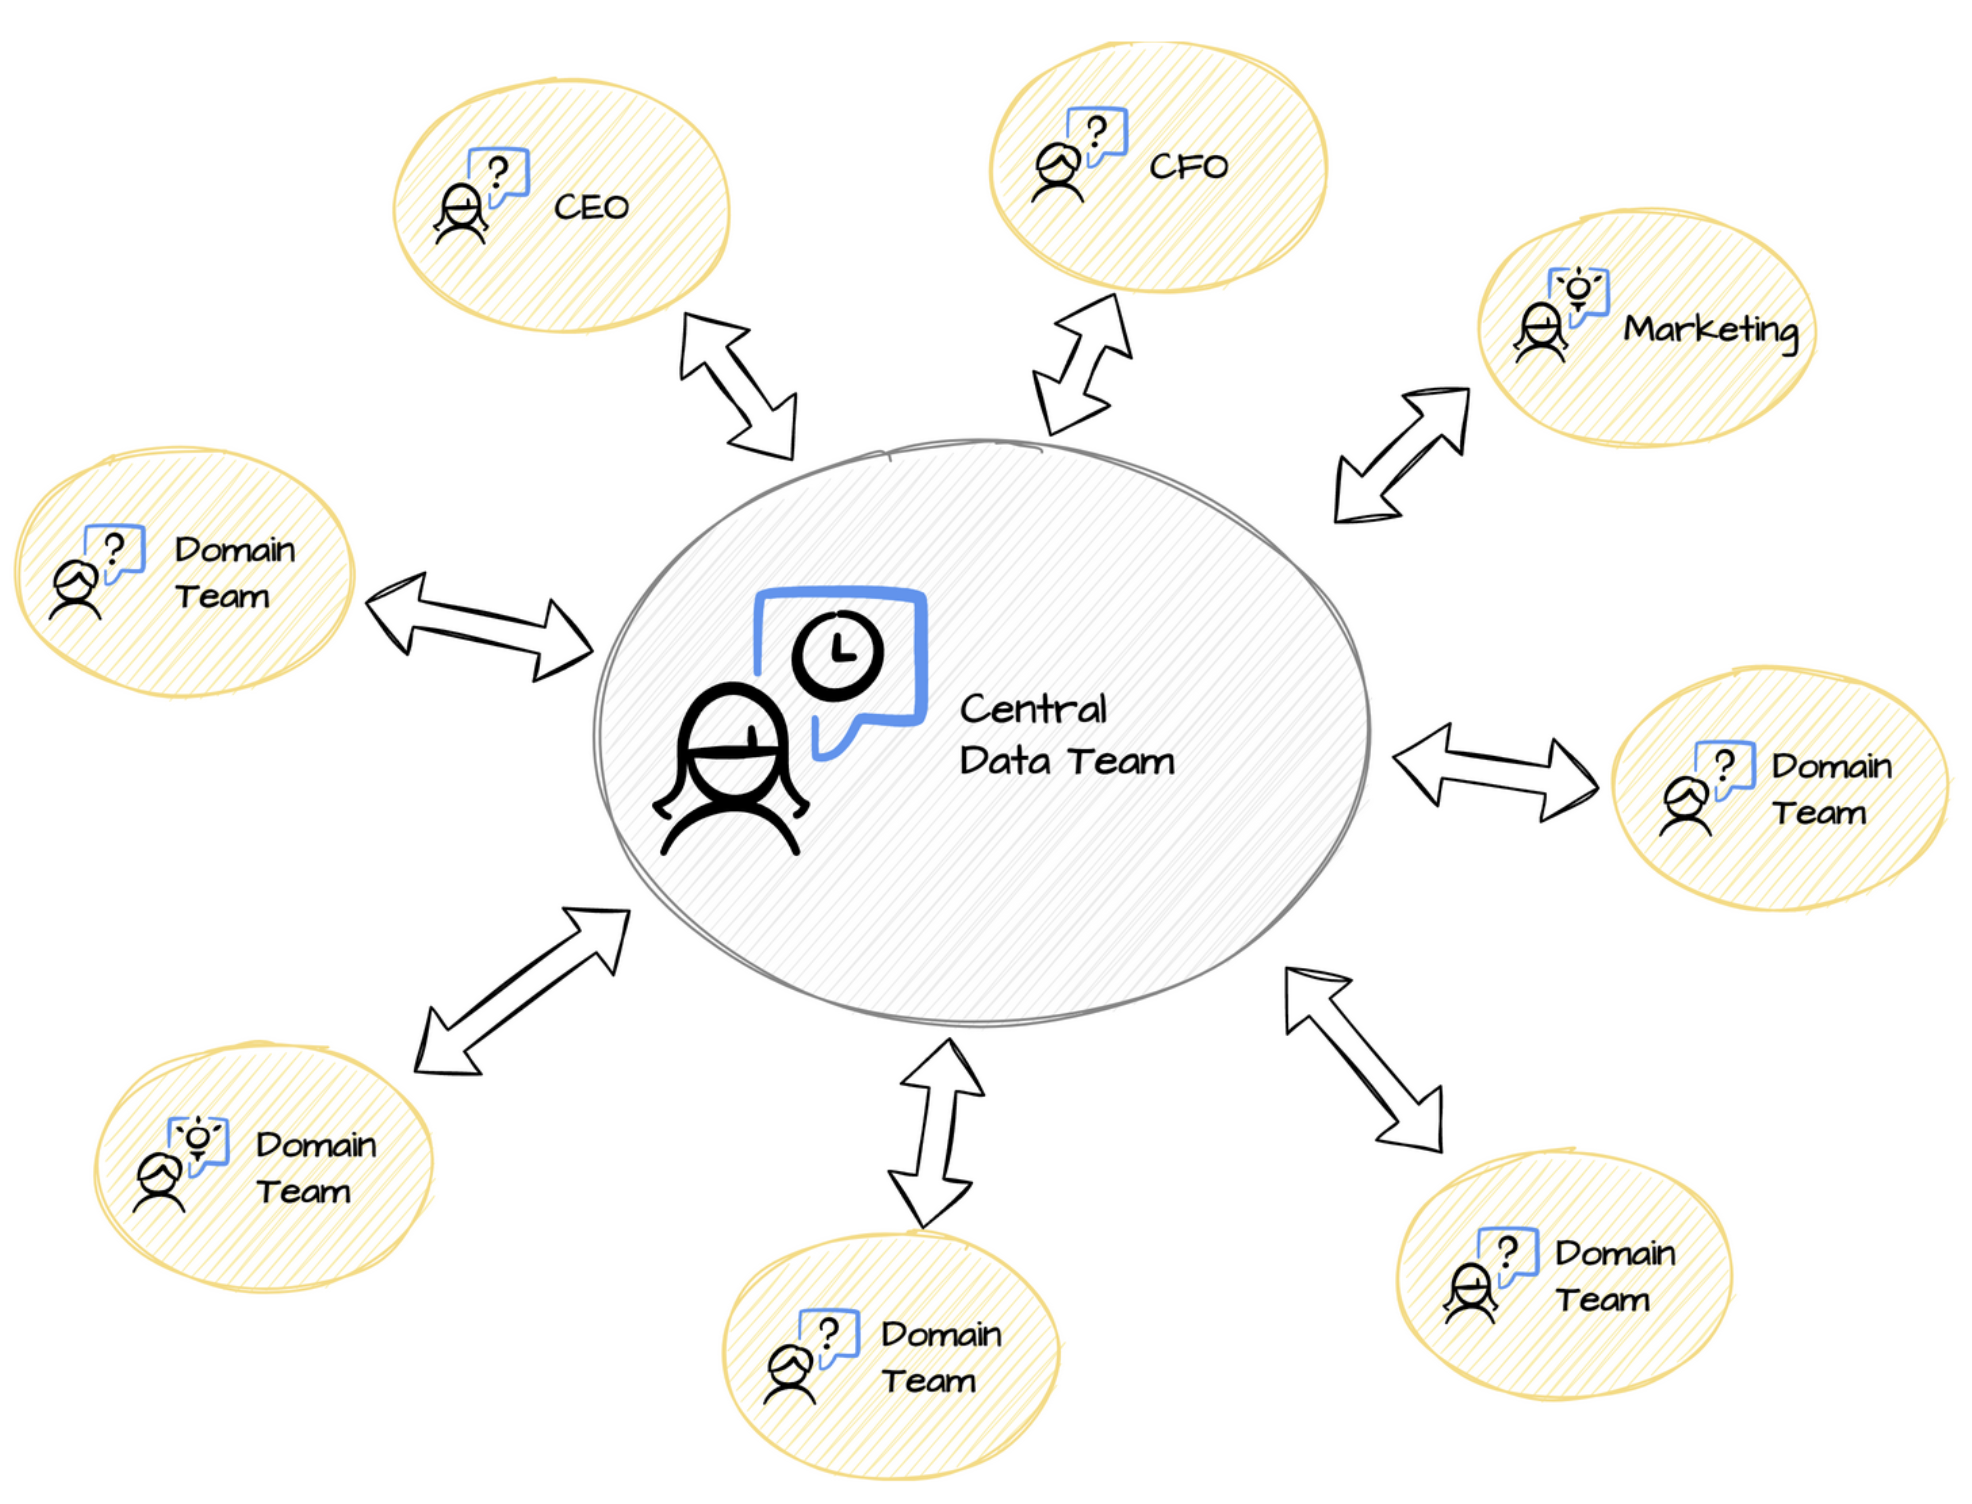
\includegraphics[width=14cm]{CentralDataTeam.png}
	\caption{Central data team in a data-driven business}
	\label{centraldata}
\end{figure}

This model works quite well at the first time, however, after a while, they noticed that \textbf{the team often became bottleneck}. The team were overloaded with thousands of tasks and questions from multiple teams, along with the requests of time and accuracy. This lead to a massive problem since the competitiveness of business depends much on the speed of analysis. For example, when we create a landing page for a new product, how does this change the influence clicking and buying rate?

But, why the response of the central data team is so slow and struggle? Actually, once the operational database changes, the team has to spend much of their time fixing the broken data pipelines. The little remaining time is insufficient for them to discover and understanding all the necessary domain data \textbf{for each question}. Getting the required domain expertise is a daunting task. \cite{datamesh2022prologue,datameshweb}

In contrast, some firms employ domain-driven design strategies that include independent domain teams and a decentralized micro-service architecture to relieve burden on the central data team. These teams exclusively control and understand their domain, including the company's information demands. The issue hasn't entirely been resolved, though. The domain teams must contact the overloaded central data team despite being aware of the key information needs and the domain, in order to obtain the essential data-driven insights. \cite{datamesh2022prologue}

\subsection{Demands from recent developments}
Let's consider the scale-up of the software development over time. When one task grow bigger and bigger, we have to decentralize it into many smaller tasks, otherwise, all the organization will overload and lost of control. Take into consideration what we have done for the scale-up of software development:
	\begin{itemize}
		\item Decentralize business into domains;
		\item Decentralize engineering into autonomous teams;
		\item Decentralize monolith into micro-services;
		\item Decentralize operations into DevOps teams.
	\end{itemize}

Hence, the next thing we need to do is scaling up data analytics by decentralizing data lake into data mesh.\cite{datameshweb}

The position between domain teams and the central data team gets worse as the organization eventually grows. Transferring data management responsibilities from the central data team to the domain teams can help. Domain-oriented decentralization for analytical data is the central notion of the data mesh concept. Similar to APIs in a micro-service design, a data mesh architecture allows domain teams to conduct cross-domain data analysis on their own and connects data.

\section{Initial approach}
\subsection{What is Data Mesh?}
The term data mesh was first stated by Zhamak Dehghani in 2019 and is based on four fundamental principles, which will be discussed in depth later:
	\begin{itemize}
		\item Principle of Domain Ownership;
		\item Principle of Data as a Product;
		\item Principle of the Self-Serve Data Platform;
		\item Principle of Federated Computational Governance.
	\end{itemize}


\subsection{What will changes after data mesh?}
Data mesh is a fresh method for business intelligence, data analysis and management that is based on an innovative distributed architecture. Along with that, data lake and data warehouse do not disappear they just become nodes in the mesh. \cite{machado2022data,shiftkpmg}

Data mesh ensures organizations to continue to apply some data lake principles, such as making immutable data available for exploration or analytical use, and data lake tooling for internal implementation of data products or as part of the shared data infrastructure. Data lake would not be the centerpiece anymore.

It is an implementation detail sub-serving the idea of domain data product as the first-class concern. The same applies to data warehouse in terms of business reporting and visualization. \cite{shiftkpmg}

Implementing a data mesh is not a purely technical project that we can implement in isolation from the rest of the business. It's not some thing that we can just start with, and then it works from the first try, but we have to grow and develop with it. It also cause a cultural shift in the organization.

\begin{figure}[h]
	\centering
	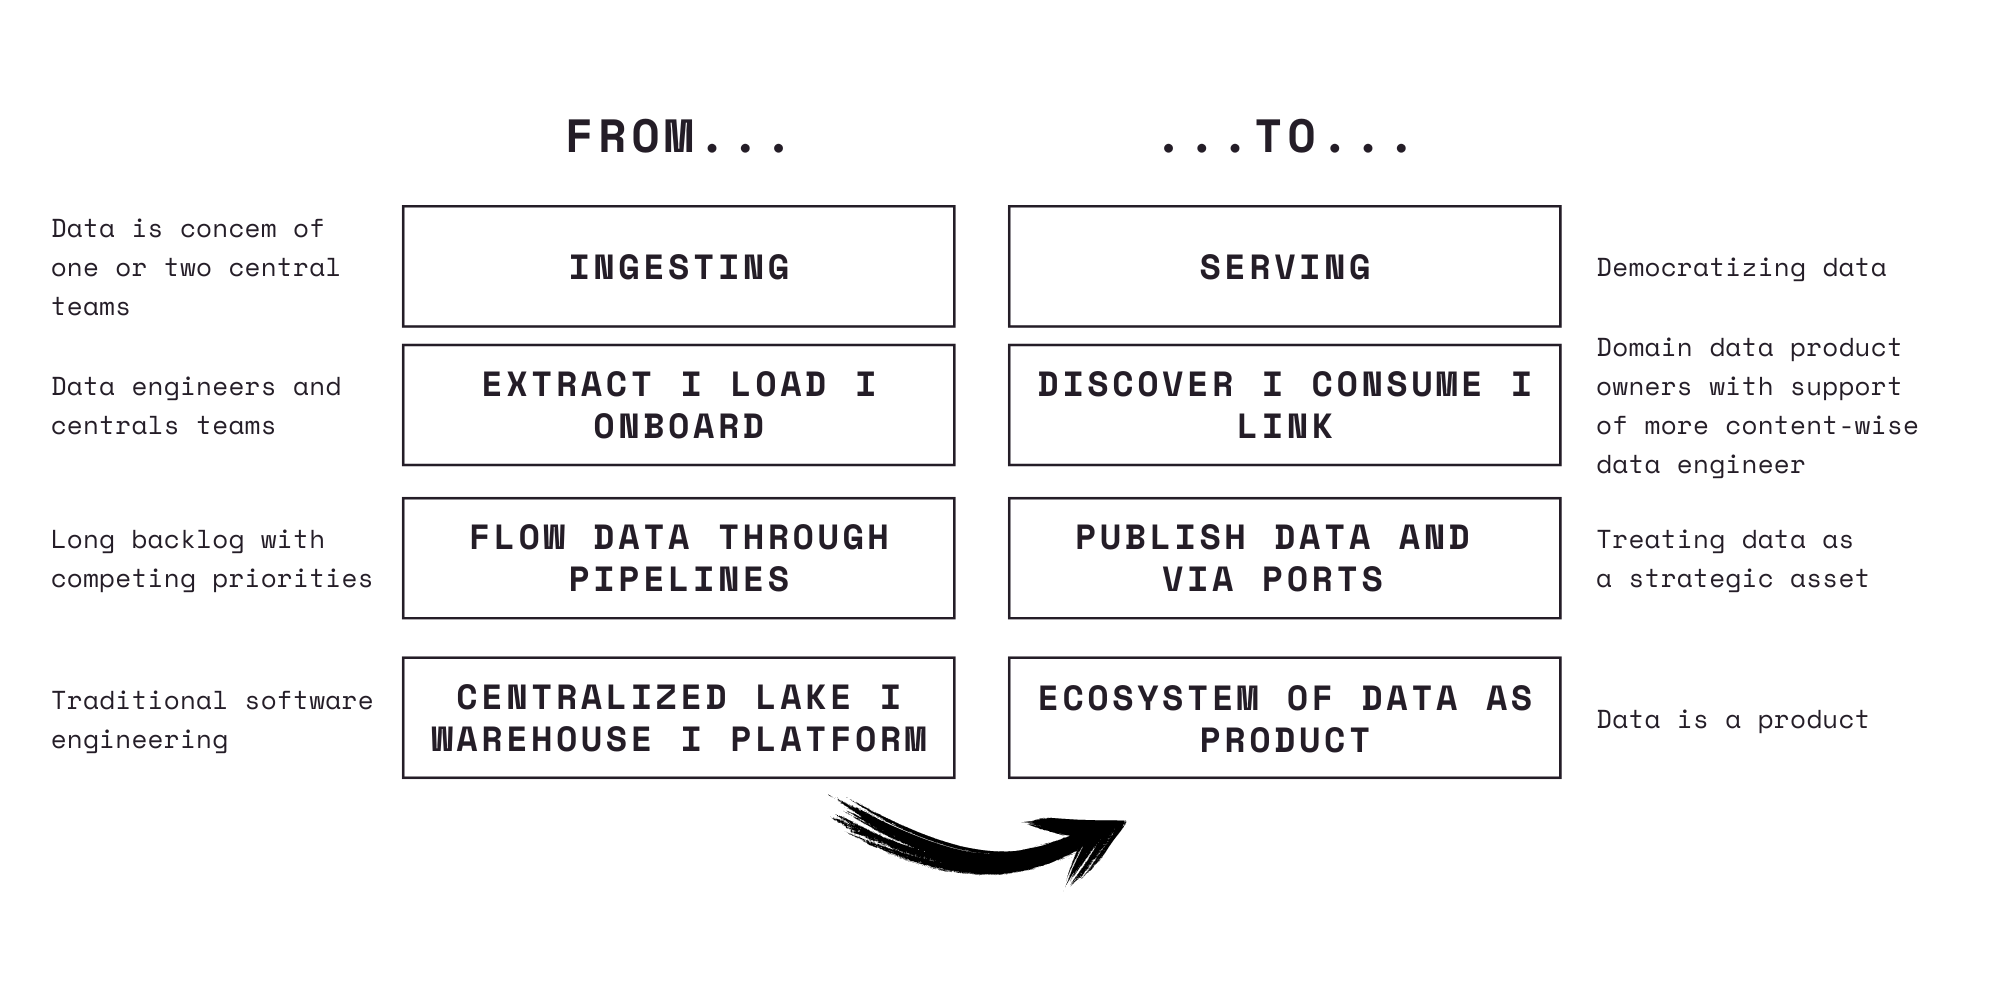
\includegraphics[width=17.5cm]{CulturalShift.png}
	\caption{Cultural shift after implementing data mesh}
	\label{culturalshift}
\end{figure}

Also, data mesh calls for a fundamental shift in the assumptions, architecture, technical solutions, and social structure of our organizations, that means, how we manage, use and own analytical data. \cite{datamesh2022ch1}

\begin{figure}[h]
	\centering
	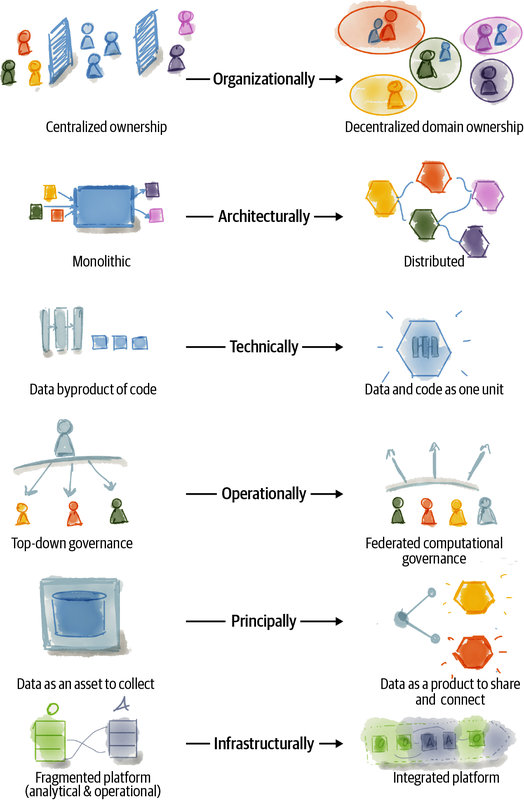
\includegraphics[width=14cm]{OrgChanges.png}
	\caption{Data mesh dimensions of organizational changes}
	\label{orgchange}
\end{figure}

Data mesh can be used as part of an enterprise data strategy, articulating the target state of the enterprise architecture as well as an organizational operating model with an iterative execution plan.

In its most basic form, it can be characterized by four interacting principles, which will be discussed in depth in section \ref{4principles}.

\chapter{Data Mesh Architecture Design}
\section{Four Fundamental Principles of Data Mesh}\label{4principles}
Four simple principles can represent the logical architecture and operating model of data mesh. They are intended to move us closer to the goals of data mesh: increasing the value of data at scale, maintaining agility as an organization grows, and embracing change in a complex and turbulent business context.

\subsection{Principle of Domain Ownership}
Data mesh, at its core, is founded in decentralization and distribution of data responsibility to people who are closest to the data. This is to support a scale-out structure and continuous and rapid change cycles.

However, in contrast to traditional data structures with technological partition (e.g. data warehouse, data lake), data mesh follows \textit{the seams of organizational units}. It follows the lines of division of responsibility aligned with the business using \textit{domain-driven design (DDD) strategies}. Data mesh also gives the data sharing responsibility yo each of the business domains, each domain is responsible for the data it is most familiar with.

\subsubsection*{Domain-Driven Design (DDD) Strategies to Data}
DDD is an approach to decomposition of software design and team allocation, based on the seams of a business. It defines a \textit{domain} as "a sphere of knowledge, influence or activity."

In data platform architecture, the closest use of DDD is for source operational systems to emit their business domain events and the monolithic data platform to consume them. DDD’s Strategic Design embraces modeling based on multiple models each contextualized to a particular domain, called a bounded context\footnote{A bounded context is the delimited applicability of a particular model that gives team members a clear and shared understanding of what has to be consistent and what can develop independently. \cite{dddevan}}. As Z. Dehghani's recommendation, data mesh adopts the boundary of bounded contexts to individual data products - data, its models, and its ownership. For some organizations have built services based on the domain bounded contexts, now, they apply the same decomposition and modeling to their analytical data in each domain.

Domain data ownership is the foundation of scale in a complex system like enterprises today. When we map the data mesh to an organization and its domains, we discover a few different archetypes of domain-oriented analytical data, then we defined them as:
	\begin{itemize}
		\item Source-aligned domain data (native data product): Analytical data reflecting the business facts generated by the operational systems.
		\item Aggregate domain data: Analytical data that is an aggregate of multiple upstream domains.
		\item Consumer-aligned (fit-for-purpose) domain data: Analytical data transformed to fit the needs of one or multiple specific use cases.
	\end{itemize}

\begin{figure}[h]
	\centering
	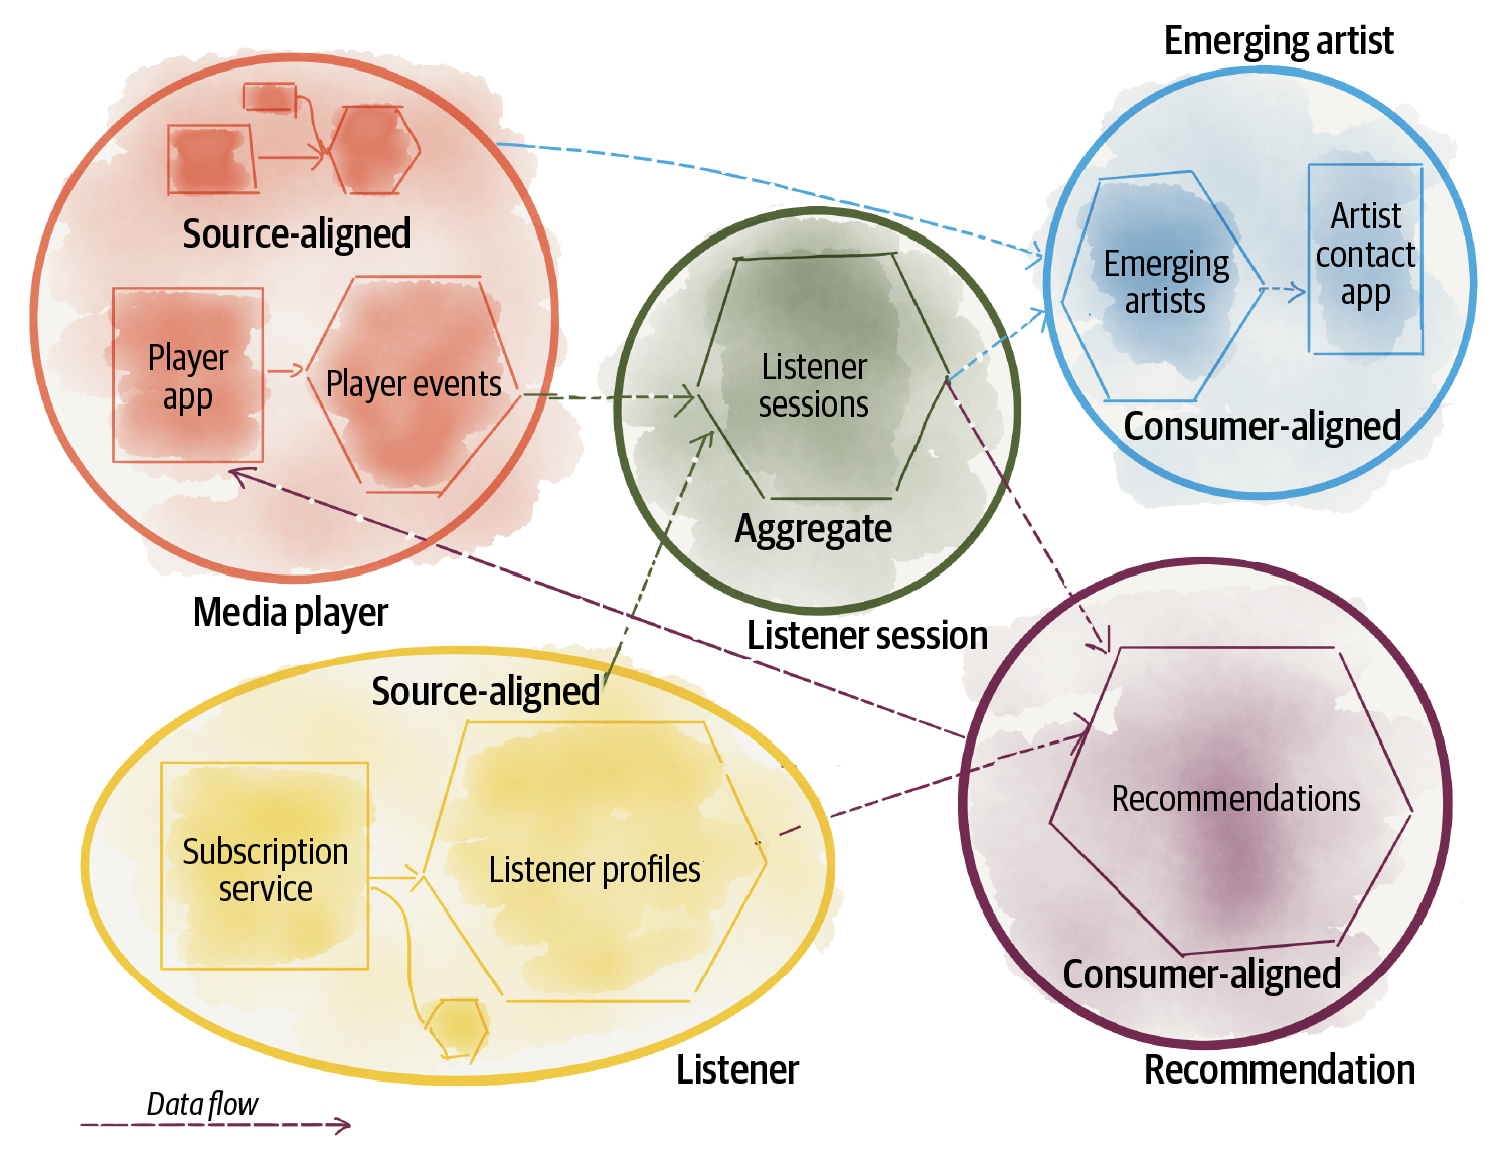
\includegraphics[width=14cm]{DecomposeData.png}
	\caption{Decomposing the analytical data ownership and architecture, aligned with business domains, along with their data archetypes.}
	\label{DecomposeData}
\end{figure}

%------ NOT STARTED-----------
\chapter{Data Product Design \& Implementation}

\chapter{Data Mesh in use}
\section{Data Mesh with Data Lakehouse}

\section{Frameworks and technologies for Data Mesh}

\section{Case study or Demo}


\begingroup
\backmatter
\pagenumbering{alph}
\renewcommand\bibname{References}

\bibliographystyle{IEEEtran} % We choose the "plain" reference style
\bibliography{includes/refs} % Entries are in the refs.bib file
\endgroup

\clearpage
\end{document}